\documentclass[../../../interview-questions.tex]{subfiles}

\begin{document}

\subsection{\color{red}{Java内存结构}}

根据JVM虚拟机规范,运行时数据区通常包括这几个部分:程序计数器(Program Counter Register)、Java栈(VM Stack)、本地方法栈(Native Method Stack)、方法区(Method Area)、堆(Heap)。为了便于记忆,可以逻辑上分为2部分,一是所有线程共享的部分,包括方法区(Method Area)和堆(Heap),二是单个线程私有的部分,包括程序计数器(Program Counter Register)、虚拟机栈(VM Stack)、本地方法栈(Native Method Stack)。Java栈中存放的是一个个的栈帧(Stack Frame),每个栈帧对应一个被调用的方法,在栈帧中包括局部变量表(Local Variables)、操作数栈(Operate Stack)、指向当前方法所属的类的运行时常量池(运行时常量池的概念在方法区部分会谈到)的引用(Reference to runtime constant pool)、方法返回地址(Return Address)和一些额外的附加信息。当线程执行一个方法时,就会随之创建一个对应的栈帧,并将建立的栈帧压栈。当方法执行完毕之后,便会将栈帧出栈。

\textbf{方法区(Method Area)}在JVM中也是一个非常重要的区域,它与堆一样,是被线程共享的区域。在方法区中,存储了每个类的信息(包括类的名称、方法信息、字段信息)、静态变量、常量以及编译器编译后的代码等。运行时常量池是方法区的一部分,用于存放编译期间生成的各种字面常量和符号引用。通过反射获取到的类型、方法名、字段名称、访问修饰符等信息就是从方法区获取到的。在使用到CGLib对类进行增强时,增强的类越多,就需要越大的方法区类存储动态生成的Class信息,当存放方法区数据的内存溢出时,会报OutOfMemoryError异常。在JDK 1.8中也就是Metaspace内存溢出,可以通过参数JVM参数-XX:MetaspaceSize和-XX:MaxMetaspaceSize设置Metaspace的空间大小。在jdk7及以前,习惯上把方法区,称为永久代。JDK 1.8后方法区(Method Area)被元空间(Metaspace)代替。JDK 1.8后,元空间存放在堆外内存中。元空间的本质和永久代类似,都是对JVM规范中方法区的实现。不过元空间与永久代最大的区别在于:元空间不在虚拟机设置的内存中,而是使用本地内存。

\textbf{堆(Heap)}Heap是OOM故障最主要的发源地,它存储着几乎所有的实例对象,堆由垃圾收集器自动回收,堆区由各子线程共享使用;通常情况下,它占用的空间是所有内存区域中最大的,但如果无节制地创建大量对象,也容易消耗完所有的空间;堆的内存空间既可以固定大小,也可运行时动态地调整,通过参数-Xms设定初始值、-Xmx设定最大值。JVM中的堆(Heap),一般分为三大部分:新生代(Young Generation)、老年代(Old Generation)、永久代(Permanent Generation):新生代又分为 Eden区、ServivorFrom、ServivorTo三个区。Eden区:Java新对象的出生地(如果新创建的对象占用内存很大,则直接分配到老年代)。当Eden区内存不够的时候就会触发MinorGC,对新生代区进行一次垃圾回收。ServivorTo:保留了一次MinorGC过程中的幸存者。ServivorFrom:上一次GC的幸存者,作为这一次GC的被扫描者。

\textbf{程序计数器(Program Counter Register)}是一个记录着当前线程所执行的字节码的行号指示器。JVM的多线程是通过CPU时间片轮转(即线程轮流切换并分配处理器执行时间)算法来实现的。也就是说,某个线程在执行过程中可能会因为时间片耗尽而被挂起,而另一个线程获取到时间片开始执行。当被挂起的线程重新获取到时间片的时候,它要想从被挂起的地方继续执行,就必须知道它上次执行到哪个位置,在JVM中,通过程序计数器来记录某个线程的字节码执行位置。因此,程序计数器是具备线程隔离的特性,也就是说,每个线程工作时都有属于自己的独立计数器。

\textbf{虚拟机栈(VM Stack)}:每个线程有一个私有的栈,随着线程的创建而创建。栈里面存着的是一种叫“栈帧”的东西,每个方法会创建一个栈帧,栈帧中存放了局部变量表(基本数据类型和对象引用)、操作数栈、方法出口等信息。栈的大小可以固定也可以动态扩展。当栈调用深度大于JVM所允许的范围,会抛出StackOverflowError的错误.

\tikzstyle{heap} = [rectangle, rounded corners, minimum width=3cm, minimum height=1cm,text centered, draw=black, fill=red!30]
\tikzstyle{heapshare} = [rectangle, rounded corners, minimum width=3cm, minimum height=1cm,text centered, draw=black, fill=red!30]
\tikzstyle{heapindependent} = [rectangle, rounded corners, minimum width=3cm, minimum height=1cm,text centered, draw=black, fill=red!30]
\tikzstyle{methodarea} = [rectangle, rounded corners, minimum width=4cm, minimum height=2cm,text centered, draw=black, fill=yellow!30]
\tikzstyle{javaheap} = [rectangle, rounded corners, minimum width=4cm, minimum height=2cm,text centered, draw=black, fill=yellow!30]
\begin{tikzpicture}
\node at (4, 0) [heap, draw=red!50, fill=red!20, text=red!70] {虚拟机栈(VM Stack)};
\node at (8, 0) [heap, draw=red!50, fill=red!20, text=red!70,text width=3cm] {本地方法栈 (Native Method Stack)};
\node at (0, 0) [heap, draw=red!50, fill=red!20, text=red!70,text width=3.5cm] {程序计数器(Program Counter Register)};
\node at (0, -2) [javaheap, draw=red!50, fill=yellow!30, text=red!70] {堆(Heap)};
\node at (5, -2) [methodarea, draw=red!50, fill=yellow!30, text=red!70] {方法区(Method Area)};
\end{tikzpicture}

\textbf{本地方法栈( Native Method Stack)}本地方法栈和虚拟机栈所发挥的作用是很相似的,它们之间的区别不过是虚拟机栈为虚拟机执行Java方法(字节码)服务,而本地方法栈则为虚拟机使用到的Native方法服务。Sun HotSpot 直接就把本地方法栈和虚拟机栈合二为一。本地方法栈也会抛出StackOverflowError和OutOfMemoryError异常。

\begin{figure}[htbp]
	\centering
	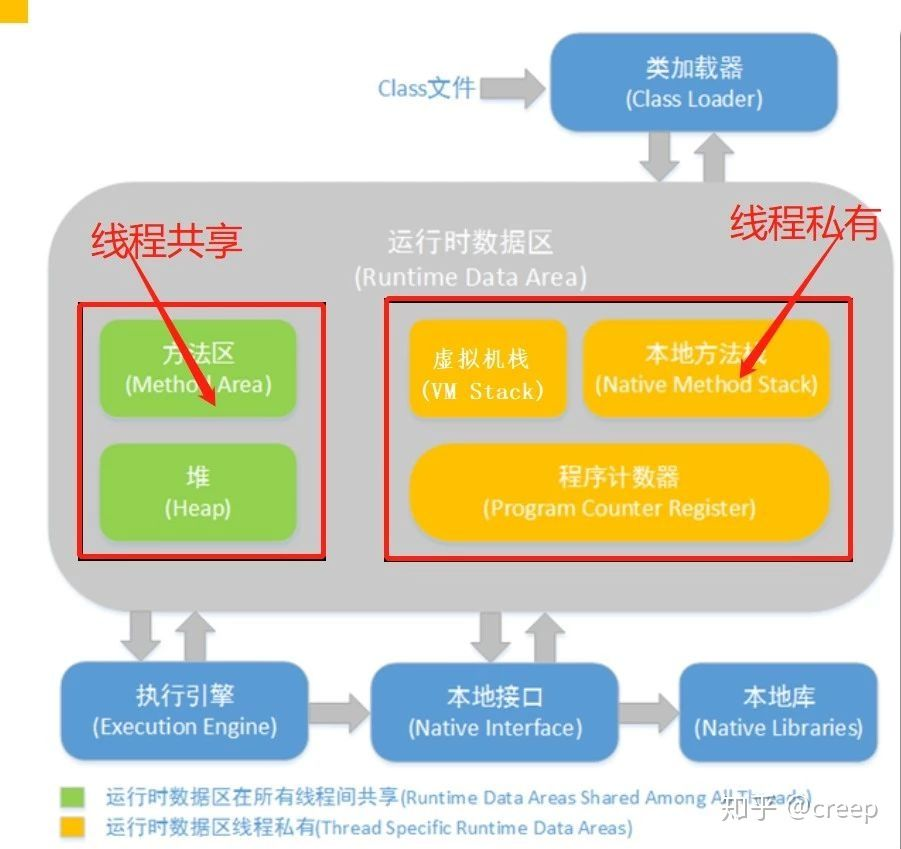
\includegraphics[scale=0.25]{jvm-memo-model.jpeg}
	\caption{JVM内存模型}
	\label{fig:collection1}
\end{figure}


\end{document}